\usetikzlibrary{calc,arrows.meta,positioning,backgrounds}
\begin{tikzpicture} [
    description/.style={draw=gray!70, thick, line cap=round, every node/.style={align=center, font=\scriptsize\sffamily, anchor=north}},
imagearrow/.style={red, line cap=round, -{Triangle[width=3*#1]}, line width=#1, shorten >=#1*0*1.75pt, every node/.append style={fill, circle, inner sep=0pt, minimum size=#1*3.5pt, anchor=center, outer sep=0pt}}
  ]

\definecolor{bluewindow}{RGB}{215,238,244}
\definecolor{bluecar}{RGB}{64,81,181}


\node[inner sep=0pt] (russell) at (0,0)
  {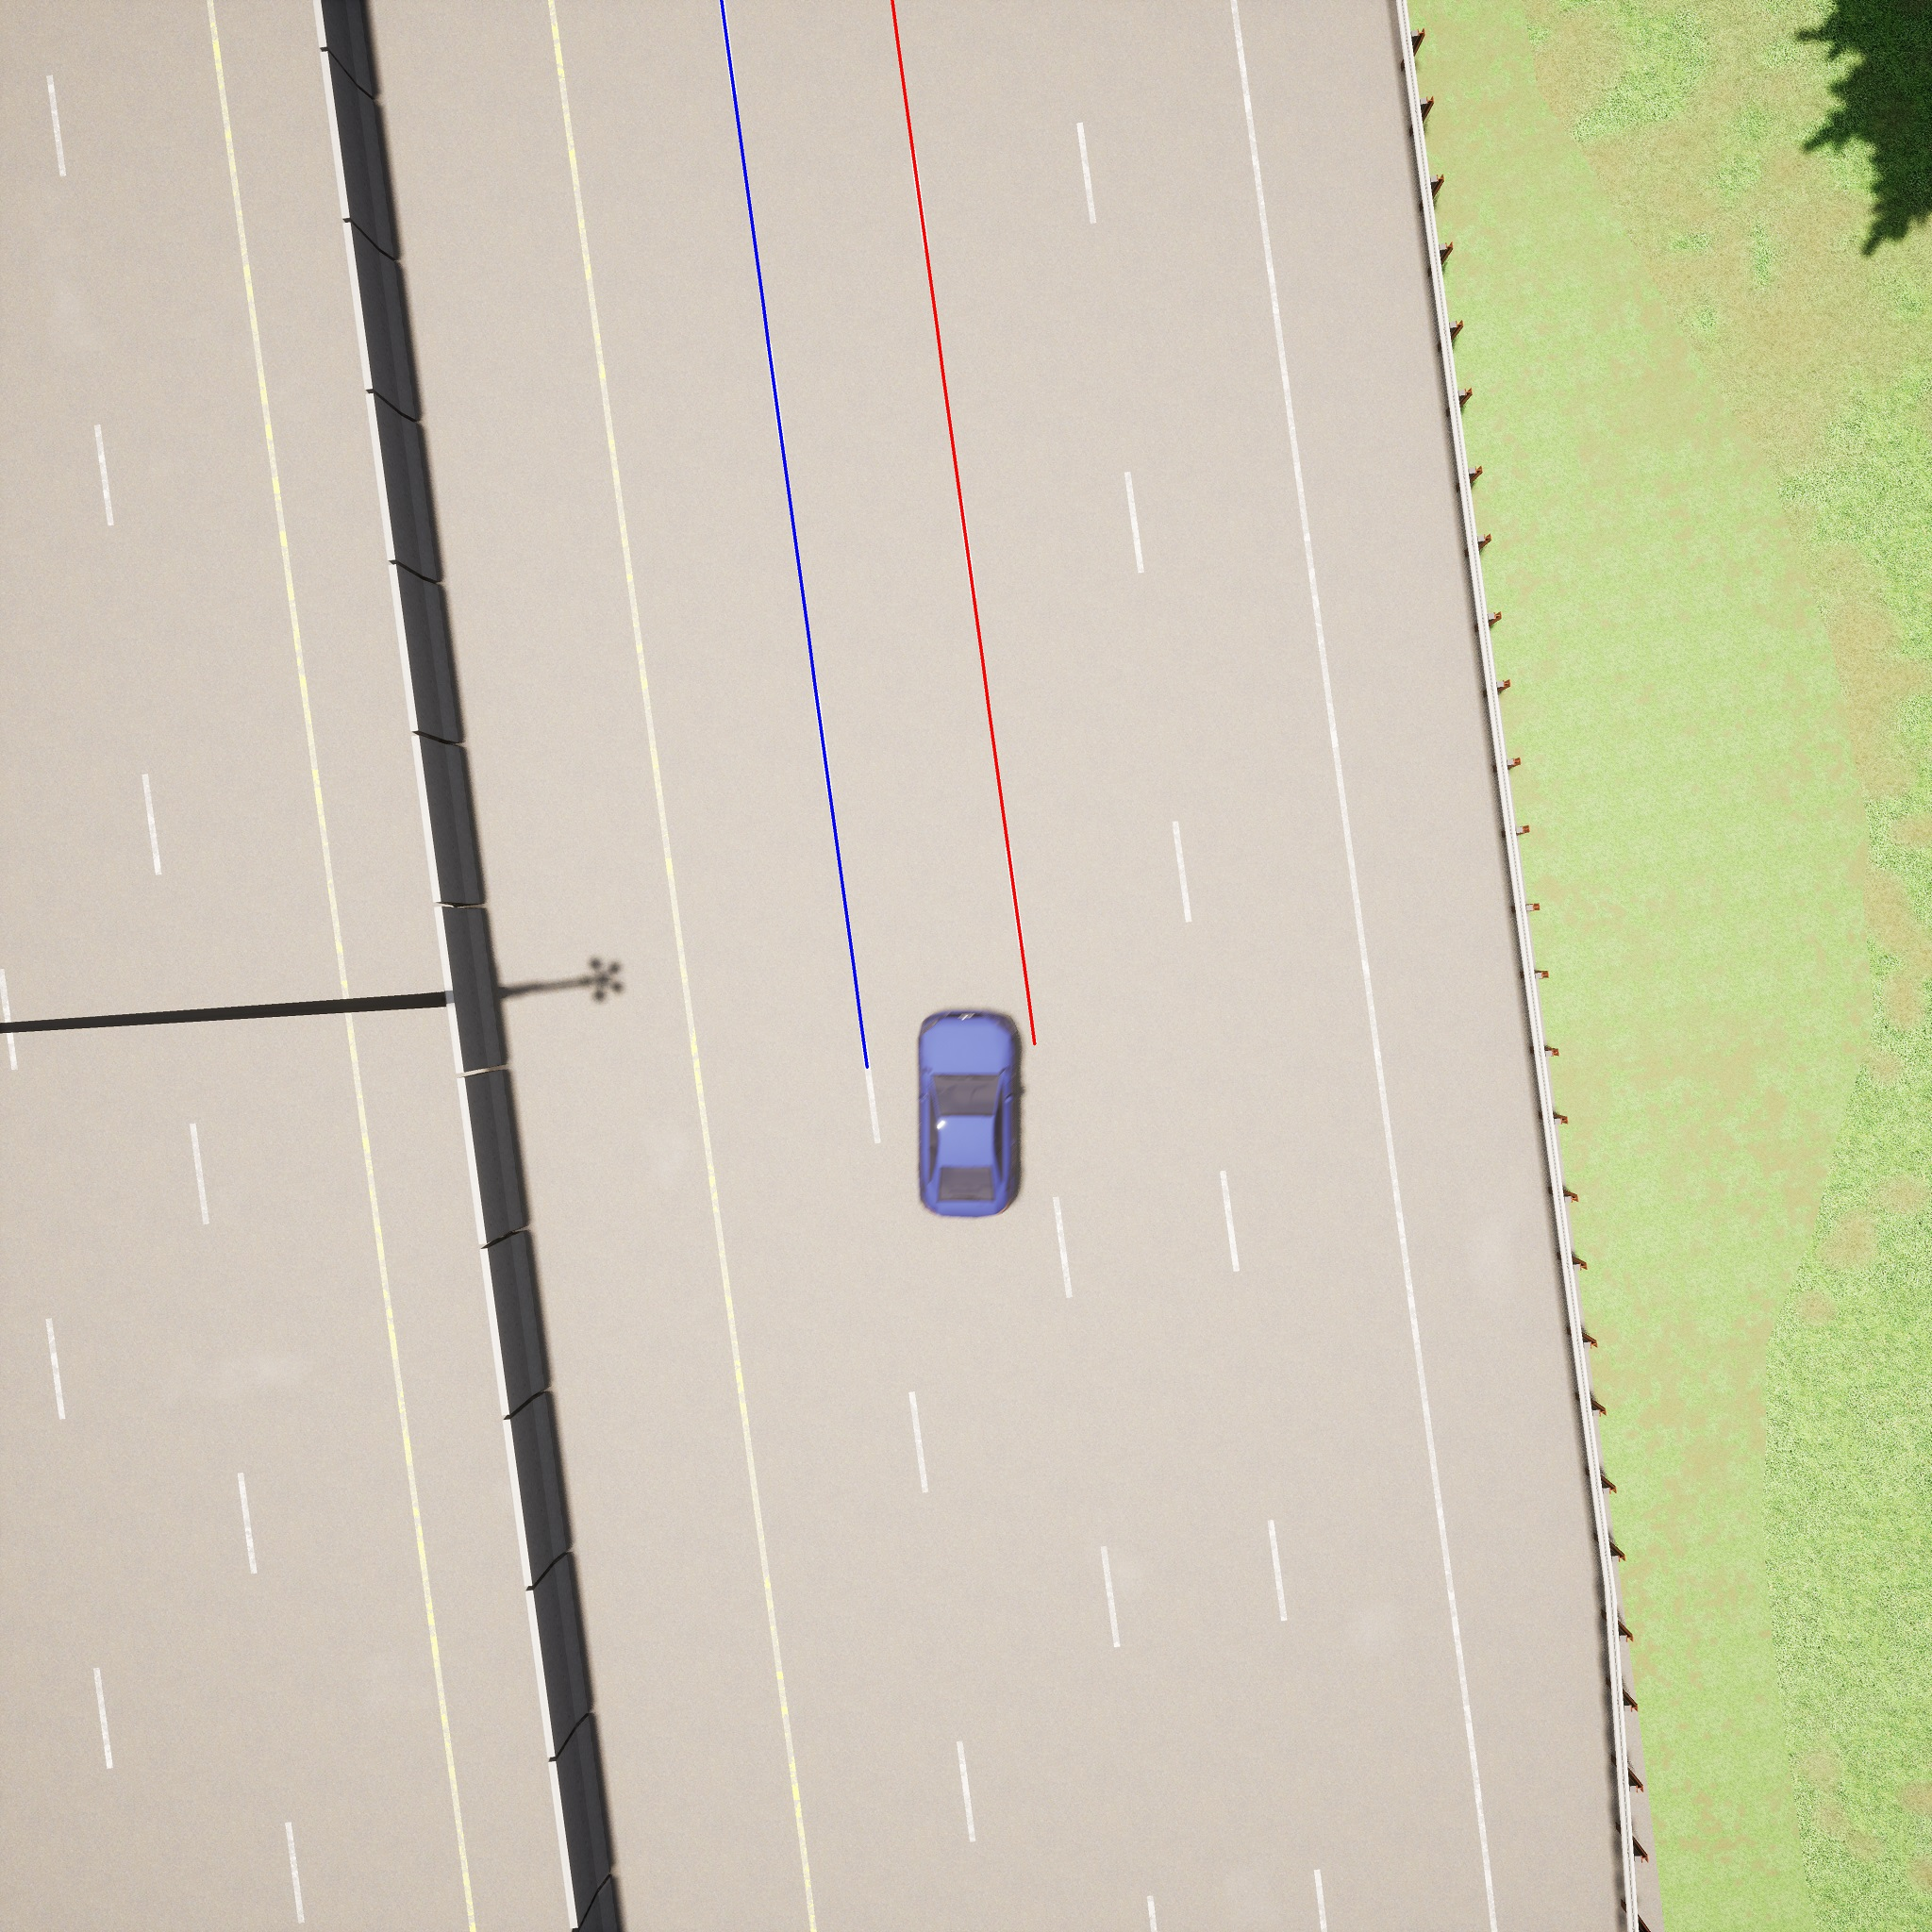
\includegraphics{bev_2.jpg}};



% define some math for coordinate axes
\pgfmathsetmacro{\len}{2.5}
\pgfmathsetmacro{\cosp}{0.94}
\pgfmathsetmacro{\sinp}{0.34}

\pgfmathsetmacro{\ocx}{2.58}
\pgfmathsetmacro{\ocy}{2.75}

\pgfmathsetmacro{\orx}{-0.06}
\pgfmathsetmacro{\ory}{-1.72}

\pgfmathsetmacro{\owx}{-11.5}
\pgfmathsetmacro{\owy}{4.4}
\pgfmathsetmacro{\eps}{0.8}


%road system
\draw[->, ultra thick] (\orx,\ory) -- (\orx, \ory+\len) node[above right]{\Huge $x$};
\draw[->, ultra thick] (\orx,\ory) -- (\orx-\len, \ory) node[below left]{\Huge $y$};

%\draw[blue] (-1.8,4) node {\Huge $y_l(x)$};
%\draw[red] (3.2,5) node {\Huge $y_r(x)$};

\draw[blue] (-3.5,4.7) node {\Huge $y_l(x)$};
\draw[red] (1.3,4.7) node {\Huge $y_r(x)$};


\end{tikzpicture}